



\begin{frame}{\citetitle{MarcoNuno_CongArbIng_2014_12_00X}  \footnotemark (1)}
\begin{columns}
\begin{column}{0.4\textwidth}
		Componentes:
		\begin{itemize}
		\item Una cama para libros abiertos
		\item Un mecanismo para cambiar de página a través de uns servomotores
		\item Un sistema de iluminación 		
		\end{itemize}
\end{column}
\begin{column}{0.6\textwidth}  
    \begin{center}
     %%%%% this is a minipage, so \textwidth is already adjusted to the size of the column
     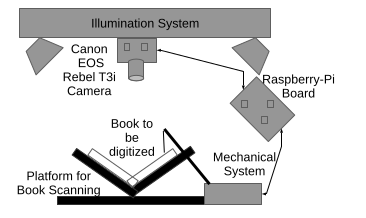
\includegraphics[width=0.8\textwidth]{Figs/BookScanner1}
     \end{center}
\end{column}
\end{columns}

\footnotetext[1]{\fullcite{MarcoNuno_CongArbIng_2014_12_00X}}
\setcounter{footnote}{0}
\end{frame}


\begin{frame}{\citetitle{MarcoNuno_CongArbIng_2014_12_00X} (2)}
%\begin{block}{Prototipo para Digitalizar Libros (2)} 
\begin{columns}
\begin{column}{0.6\textwidth}
		\begin{itemize}
		\item Una cámara de alta definición para capturar fotografías de ambas páginas
		\item Una computadora Embebida con la cámara conectada para procesar la imágen e integrar el libro digitalizado en formato PDF.
		\item Nucleo: Un sistema de visión para detectar automáticamente los límites de las páginas y cortas para generar el documento
		\end{itemize}
\end{column}
\begin{column}{0.4\textwidth}  
    \begin{center}
     %%%%% this is a minipage, so \textwidth is already adjusted to the size of the column
     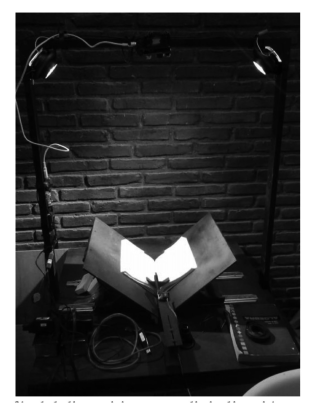
\includegraphics[width=0.8\textwidth]{Figs/BookScanner2}
     \end{center}
\end{column}
\end{columns}
%\end{block} 
\end{frame}


\begin{frame}{\citetitle{MarcoNuno_CongArbIng_2014_12_00X} (3)}
%\begin{block}{} 
\begin{columns}
\begin{column}{0.5\textwidth}
%   some text here some text here some text here some text here some text here
     \begin{center}
     %%%%% this is a minipage, so \textwidth is already adjusted to the size of the column
     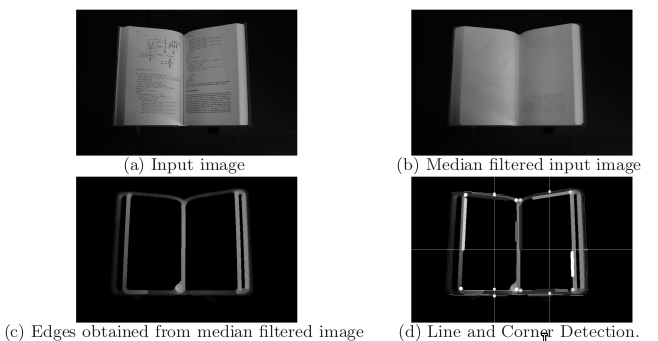
\includegraphics[width=0.88\textwidth]{Figs/BookScanner3}
     \end{center}

\end{column}
\begin{column}{0.5\textwidth}  
    \begin{center}
     %%%%% this is a minipage, so \textwidth is already adjusted to the size of the column
     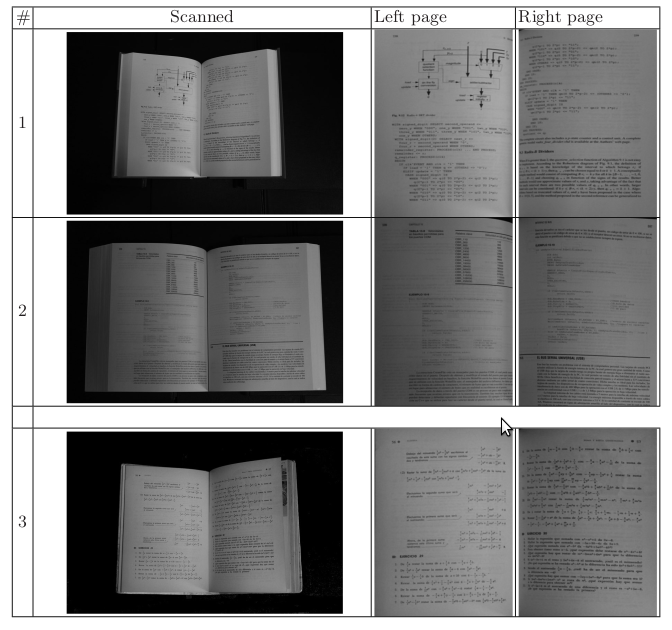
\includegraphics[width=0.88\textwidth]{Figs/BookScanner4}
     \end{center}
\end{column}
\end{columns}
%\end{block} 
\end{frame}


